\documentclass{IAYCPro}

\projectyear{2024}
\projectauthor{\large Konstantinos Kilmetis (s3745597) \& Diederick Vroom (s2277387)}
\projectname{Computational Physics: The Ising Model}
\projectgroup{COP 2024}

\projectstartpage{1}
\usepackage[latin1]{inputenc}
\usepackage[english]{babel}
\usepackage{gensymb}
\usepackage{graphicx}
\usepackage{verbatim}
\usepackage{wasysym}
\usepackage{marvosym}
\usepackage{lmodern}
\usepackage{hyperref}
\usepackage{siunitx} %\si{km.s^{-1}} unit
\usepackage{mathtools} %\Aboxed{} for box
\usepackage{chngcntr} %For using split environment --> give equations in align environment 1 reference label
\counterwithout{equation}{section} %Count equation labels independently of section numbers. I.e. no longer equation (3.14) (equation 14 in section 3), instead it is a whole number, e.g. equation (42) (42nd equation in the entire document).
\usepackage{multirow}
\usepackage{subcaption}

\newcommand{\dd}{\mathrm{d}} %For easily writing differentials
\newcommand{\ssi}[1]{\;\si{#1}} %automatically put a space before using units with \si{}

% Fonts
\usepackage{fontspec}
\newfontfamily\droid[
  Path = fonts/ ,
  UprightFont = *-Regular,
  BoldFont = *-Bold,
  ItalicFont = *-Italic,
  BoldItalicFont = *-BoldItalic,
  Extension = .ttf
  ]{DroidSerif}
\setmainfont{DroidSerif}
\usepackage{listings}

%This is a skeleton file for typesetting source code ---using the LaTeX listings package--- for the Computational Physics course 2019-2020.
%Tested and compiles using pdflatex, lualatex and xelatex.

%The following settings are copied from Wikibooks (https://en.wikibooks.org/wiki/LaTeX/Source_Code_Listings) and slightly adjusted:
\lstset{ 
  backgroundcolor=\color{white},   % choose the background color; you must add \usepackage{color} or \usepackage{xcolor}; should come as last argument
  basicstyle=\footnotesize,        % the size of the fonts that are used for the code
  breakatwhitespace=true,          % sets if automatic breaks should only happen at whitespace
  breaklines=true,                 % sets automatic line breaking
  linewidth=\linewidth,            % sets the linewidth of the code frame to the linewidth of the document
  commentstyle=\color{gray}\itshape, % make comments gray and italic 
  captionpos=b,                    % sets the caption-position to bottom
  deletekeywords={...},            % if you want to delete keywords from the given language
  escapeinside={\%*}{*)},          % if you want to add LaTeX within your code
  extendedchars=true,              % lets you use non-ASCII characters; for 8-bits encodings only, does not work with UTF-8
  firstnumber=1,                   % start line enumeration with line 1000
  frame=single,	                   % adds a frame around the code
  keepspaces=true,                 % keeps spaces in text, useful for keeping indentation of code (possibly needs columns=flexible)
  language=Python,                 % the language of the code
  morekeywords={as, self, Dict, Tuple, List, Any, Union, None, ...},            % if you want to add more keywords to the set
  numbers=left,                    % where to put the line-numbers; possible values are (none, left, right)
  numberstyle=\tiny,               % line numbers are smaller
  numbersep=5pt,                   % how far the line-numbers are from the code
  rulecolor=\color{black},         % if not set, the frame-color may be changed on line-breaks within not-black text (e.g. comments (green here))
  showspaces=false,                % show spaces everywhere adding particular underscores; it overrides 'showstringspaces'
  showstringspaces=false,          % underline spaces within strings only
  stringstyle=\color{gray},        % strings are also gray
  showtabs=false,                  % show tabs within strings adding particular underscores
  stepnumber=1,                    % the step between two line-numbers. If it's 1, each line will be numbered
  tabsize=2,	                   % sets default tabsize to 2 spaces
  title=\lstname                   % show the filename of files included with \lstinputlisting; also try caption instead of title
}

\begin{document}
\begin{center}
    \textbf{Abstract}
\end{center}
\vspace{-1em}
    We numerically solve the two dimensional Ising model for a square crystal composed of 50$\times$50 spins with periodic boundary conditions. We observe the phase transition at approximately where it is theoretically predicted, $T_\mathrm{C}$ = $2J/\ln\left(1 + \sqrt{2}\right)$. We extend our investigation by embedding the crystal in various external magnetic fields. Their presence changes the value of $T_\mathrm{C}$, scaling with the strengths of the magnetic fields. 
\section{Introduction}
\label{sct: Introduction}
Magnets are the closest thing to magic accessible to humans. They are materials which under certain circumstances have the property to attract and repulse other materials. The responsible force is electromagnetism, but unlike pure electrostatics, the nature of a magnet is more complex than a charge distribution. In electrostatics, a scalar property, charge density, describes the strength of the interaction, whereas in magneto-statics  the interaction is governed by the stochastic interactions between a magnet's constituent parts.\\ \\
The specific sort of magnet we will examine, ferromagnets, has a magnetic field because each one of its constituent parts possess a magnetic spin. These spins can be thought of as vectors of equal magnitudes but different direction. In ferromagnetic materials the directions of these spins happen to align which leads to a permanent, large scale magnetic field.

\begin{figure}[H]
    \centering
    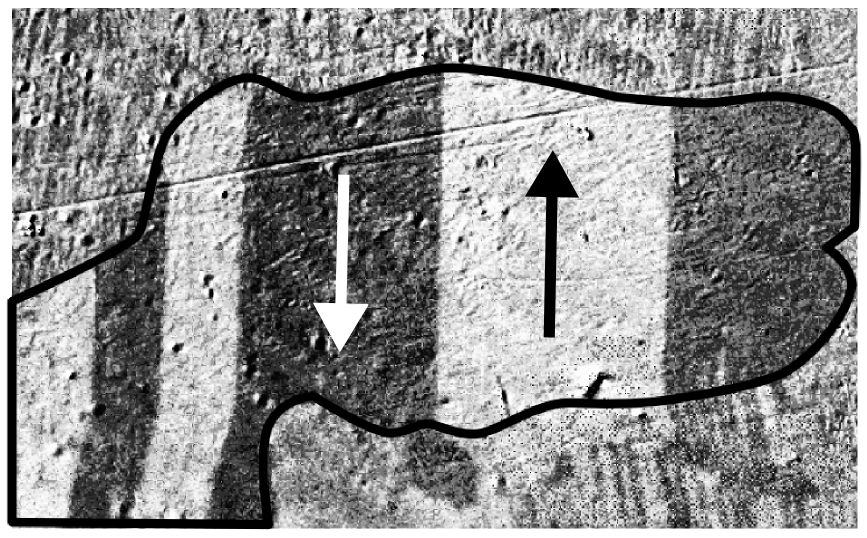
\includegraphics[scale = 0.25]{figs/magdomain.png}
    \caption[fuck]{\small{Magnetic domains in a single grain (outlined with a black line) of non-oriented electrical steel, photographed under Kerr-effect microscope. The arrows show the direction of magnetisation in each domain - all white domains are magnetised "up", all dark domains are magnetised "down".
    Image \& Caption source: Wikimedia Commons\footnotemark }}
    \label{fig:domain}
\end{figure}

\footnotetext{\href{https://commons.wikimedia.org/wiki/File:Magnetic_domain_with_arrows_by_Zureks.png}{\texttt{https://commons.wikimedia.org/wiki/File:Magnetic\_domain\_with\_arrows\_by\_Zureks.png}}}

\raggedbottom
\newpage


Each spin acts on its neighbours, trying to align their spin with its own. As a result, magnetic domains emerge; parts of the material where one orientation dominates, minimising the energy of the system. This \textit{conformal} force is opposed by the tendency magnets have to flip. This polarity flip occurs not only in small scale materials but has been observed in both the magnetic field of the Earth and that of the Sun\footnote{Both of these systems are not static and are hosts of an ongoing dynamo process, they are only brought up as an example of polarity flip.}. Any constituent particle of the ferromagnet might flip its spin. This process is regulated by the ambient temperature. A higher temperature will make spins more likely to flip. After a critical temperature, known as the Curie temperature $T_\mathrm{C}$, the ability of spins to keep their neighbours in line ceases, discontinuously. The material then undergoes a phase transition, losing its permanent magnetic properties. This interaction is described by the Hamiltonian,

\begin{equation}
    \mathcal{H} = -J\sum_{\langle i,j\rangle} s_is_j,\; J>0,
\end{equation}

where $J$ is the coupling strength between spins and the summation goes over each spin-pair $(s_i,s_j)$. At any point, the system tries to minimise its energy. For low temperatures, the lowest energy state corresponds with an organised, low-entropy state; all spins are aligned. For temperatures greater than $T_\mathrm{C}$ , the entropy of the lowest-energy state increases with temperature.\\
Regardless of that, should the ferromagnet be embedded in an external magnetic field $\vec{H}$, the spins will try to conform not only to the their neighbours, but to the external field as well. This adds an extra term to the Hamiltonian,

\begin{equation}
    \mathcal{H} = -J\sum_{\langle i,j\rangle} s_is_j - H \sum_i s_i ,
    \label{eqn: Hamiltonian}
\end{equation}

where $H$ gives the strength of the magnetic field $\vec{H}$ perpendicular to the surface of the ferromagnet. Note: $H$ can be negative to indicate direction. The aim of this project is to computationally model a ferromagnet, and have it successfully exhibit a phase transition. After the system equilibrates, we will measure the average magnetisation. Also, we seek to measure its heat capacity and magnetic susceptibility for different temperatures. As an additional goal, we chose to investigate the behaviour of the system in the presence of an external magnetic field of different strengths.

\section{Methods}
\label{sct: Methods}

We will model a ferromagnetic material as a two-dimensional, square lattice composed of 50 particles (hereafter referred to as spins) per side. That is 2500 total spins. Of course, a real ferromagnet is composed by impossibly more spins,  we address that through implementing periodic boundary conditions. Whenever we calculate the energy of a spin sitting on the edge of our lattice, we use the spin on the opposite edge. 

\raggedbottom
\newpage

We assume that a spin only interacts with its four direct neighbours. The spins on its immediate right, left, above and below it. The 1D-version of this problem was first analytically solved by its namesake, Ernst Ising, in 1925 \cite{Ising}.

\subsection{Metropolis-Hastings algorithm}
In order to simulate the system, we utilised the Metropolis-Hastings algorithm \cite{Hastings, Metropolis}. We initialise the lattice with either 75\% positive, or 75\% negative spins. This results in quicker equilibration by avoiding local minima of the energy that occur with a random initialisation. In the random initialisation case, magnetic domains can end up being not too dissimilar to the ones in Fig. \ref{fig:domain}. This arrangement is a local minimum of the system, since only spins close to the domain boundaries are ever going to flip. The system does eventually converge by itself\footnote{We tried to be fancy here by kicking the system or annealing it. Turns out, nothing beats good ol' brute force.}, but at a significantly greater computational cost.
\\
We employed a Monte-Carlo approach; at every step, we randomly choose a spin and attempted to flip it. Then, we calculated the resulting difference in the energy. This can be done in a multitude of ways, either through a direct convolution, a Fourier transform, or analytically. The first two approaches accomplish the same thing, they convolve a kernel through the entire lattice. The kernel contains the interaction information, when considering only direct neighbours, it takes the form,

\begin{equation}
    K = \left[\begin{array}{ccc}
         0 & 1 & 0 \\
         1 & 0 & 1 \\
         0 & 1 & 0
    \end{array}
    \right],
\end{equation}

taking into account the neighbours left, right, above, and below the flipped spin. The flipped spin is the element $(1,1)$, which, of course, can not interact with itself. \\ 
For a large amount of spins, using a Fourier transform instead of a convolution, is preferable, since the fast Fourier transform scales as $\mathcal{O}(n\log n)$ and a standard convolution scales as $\mathcal{O}(n^2)$. In our case a standard convolution remains more efficient.

\raggedbottom
\newpage

\begin{figure}[H]
    \centering
    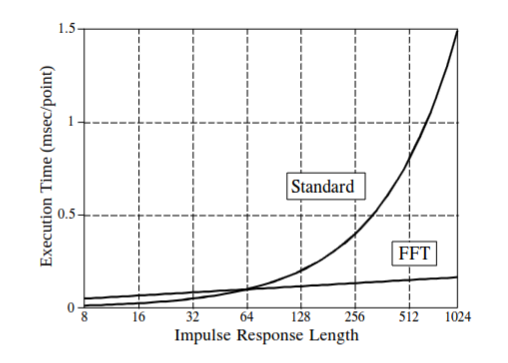
\includegraphics[scale = 0.9]{figs/fftvsnormal.png}
    \caption{The scaling of standard and FFT convolutions \small Source: Smith (2003) \cite{smith2003digital}}
    \label{fig:enter-label}
\end{figure}

Despite that, we opted for an analytical approach. Utilising the fact that only one spin flips at any given time, we can prove\footnote{See Appendix \ref{sec: Proof}.} that the energy difference $\Delta E$ is,

\begin{equation}
    \mathcal{H}^{\prime}-\mathcal{H}=2\left[ J \left(s_l+s_r+s_t+s_b\right)+ H\right]s_k,
    \label{eqn: Energy Difference}
\end{equation}

where $s_k$ is the flipped spin and $s_l$, $s_r$, $s_t$, $s_b$ are its left, right, top and bottom neighbours, respectively. This scheme allows for a scaling of $\mathcal{O}(n)$ and is easily accelerated through the \texttt{python}-package \texttt{numba} \cite{lam2015numba}. Should the total energy be reduced, we accept the new configuration. Otherwise, we utilise the energy difference to calculate the probability that this new configuration is accepted,

\begin{equation}
    P_\mathrm{accept} = e^{-\beta\Delta E}, \; \beta = \frac{1}{k_\mathrm{B}T},
\end{equation}

where $T$ is the temperature of the lattice. We achieve equilibration when the relative shift in mean energy over two equal-sized time periods is within $10^{-3}$ of each other, or the absolute shift is within $10^{-4}$ of each other. After equilibration is achieved, we continue simulating the system for enough time to ensure we can make statistically significant observations.

\raggedbottom
\newpage

\subsection{Observables}

If we wish to gather statistically significant values for our desired observables, we need to measure our systems a sufficient number of times. Of course, what we could do is let our systems continue to go through the Metropolis-Hastings algorithm an absurd number of Monte-Carlo steps and use the values in those steps to determine our observables. However, one big problem with this method is the dependency of any iteration of the lattice to previous iterations, making continuous measurements not truly independent, and are therefore biased. The way to circumvent this problem is to only measure at intervals when the lattice has completely 'forgotten' an iteration in the past. The time it takes for a system to do this is the auto-correlation time $\tau$. 

\subsubsection{Auto-Correlation Time}

We can compute the auto-correlation time by measuring how a property of the system (we will use the mean magnetisation $m$) differs from the mean $\langle m \rangle$ at some time $t$ and $t'$. This gives us the $\chi$-function,

\begin{equation}
    \chi(t) = \frac{1}{\Delta t}\sum_{t'=0}^{\Delta t} m(t')m(t'+t) - \frac{1}{\Delta t^2} \sum_{t'=0}^{\Delta t} m(t')\sum_{t'=0}^{\Delta t}m(t'+t),
\end{equation}

where $\Delta t = t_\mathrm{max} - t$ and $t_\mathrm{max}$ is the maximum time of the simulation. This function can be implemented into \texttt{python}-code in the following way:
\\
\lstinputlisting{chi.py} 

If we compute $\chi(t)$ for each simulation step \textit{after equilibration} we will see that, approximately up to the point where $\chi(t)$ first becomes negative, it can be roughly described by an exponential decay,

\begin{equation}
    \chi(t) \approx \chi_0 e^{-t/\tau},
\end{equation}

where the auto-correlation time $\tau$ plays the role of the decay time. The point where $\chi(t)$ first becomes negative signals that future values of $\chi$ are calculated using too few samples of $m$, and are thus unreliable. 

We can thus get $\tau$ by fitting an exponential decay to the $\chi$-data up to the point where $\chi$ first becomes negative. A caveat is that $\tau$ is different for each simulation at each temperature and hence we need to determine it each simulation. Using the auto-correlation time as a unit time we then measure our observables in blocks of $16\tau$ simulation steps to ensure we properly estimate the fluctuations in the observables. 

\raggedbottom
\newpage

\subsubsection{Measuring Quantities}
Measuring the average magnetisation $\langle m \rangle$ and energy $e$ are straight forward. We keep track of the total magnetisation and energy after every step. We divide by the total number of spins $N^2$, where $N=$ 50, to get the average for the lattice. The equations for these relations are given in Eqn. \ref{eqn: m and e}.

\begin{equation}
\langle | m | \rangle = \frac{1}{N^2}\left\langle\left| \sum_{i}s_i\right|\right\rangle,\quad     e = \frac{E}{N^2}.
\label{eqn: m and e}
\end{equation}

To calculate the standard deviations on the observables, we use the auto-correlation time $\tau$ and maximum time of the simulation $t_\mathrm{max}$,

\begin{equation}
    \sigma_m = \sqrt{\frac{2\tau}{t_\mathrm{max}} (\langle m^2 \rangle - \langle m\rangle^2)}.
\label{eq:sigma}
\end{equation}

In order to calculate the magnetic susceptibility $\chi_M$ (see Eqn. \ref{eqn: chi_M and C}), that is how receptive the ferromagnet is to an external field, and the specific heat capacity $C$ (see Eqn. \ref{eqn: chi_M and C}) we need to calculate the variance of the magnetisation and the energy. To do this, we split our time-domain data in chunks, each 16 auto-correlation times long. This is the reason we need to run the simulation after equilibration has been achieved. Their standard deviations are calculated using the classical statistical method.

\begin{equation}
    \chi_M = \frac{\beta}{N^2}\left(\langle M^2\rangle - \langle M \rangle^2\right),\quad 
    C = \frac{1}{N^2k_\mathrm{B}T^2}\left(\langle E^2\rangle - \langle E \rangle^2\right)
    \label{eqn: chi_M and C}
\end{equation}

\raggedbottom
\newpage

\section{Results}
\label{sct: Results}

We simulated the system for temperatures ranging from 0 to 4, with a spacing of 0.1. The average magnetisation of the system can be seen in Fig. \ref{fig:pitchfork}.

\begin{figure}[H]
    \centering
    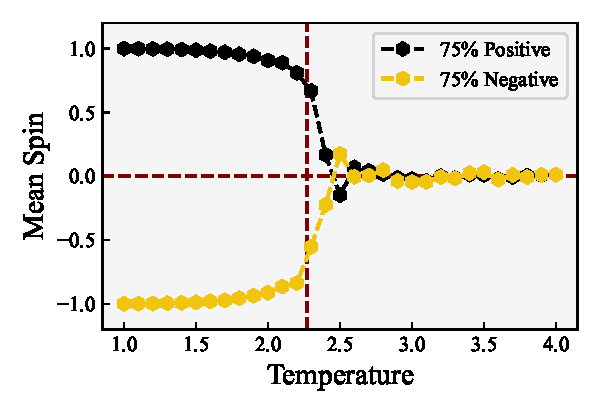
\includegraphics[width=0.7\textwidth]{figs/Pitchfork.pdf}
    \caption{Mean spin versus temperature plot, run for both a 75\% positive spin initial grid and a 75\% negative spin initial grid. The mean spins were calculated after equilibration. The vertical maroon-dashed line indicates the critical temperature $T_\mathrm{C}$ and the horizontal maroon-dashed line indicates 0 mean spin.}
    \label{fig:pitchfork}
\end{figure}

Regardless of the initialisation of the lattice, we observe the phase transition at the exact same temperature value. For low temperatures, the ferrogmagnet reaches the high-entropy, global minimum state of total conformity. It always tends to the polarity for which it was imbalanced. The final, equilibrated states of 3 example lattices are shown in Fig. \ref{fig:grids}.

\begin{figure}[H]
    \centering
    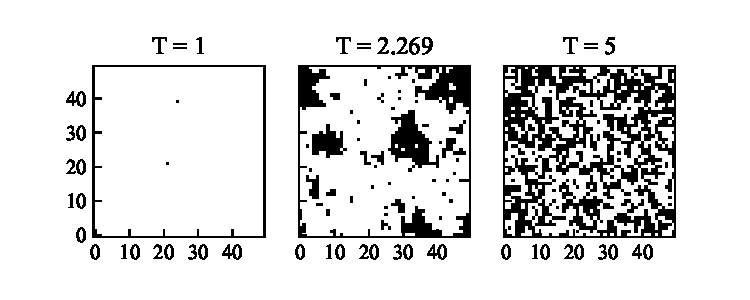
\includegraphics[width=0.7\textwidth]{figs/3Grids.pdf}
    \caption{The final state of the lattice for three temperatures. Black pixels are negative spin, white pixels are positive spin. The left panel is much lower than the critical temperature, the right panel is much higher than the critical temperature and the middle one is exactly at the critical temperature. }
    \label{fig:grids}
\end{figure}

\raggedbottom
\newpage

We present the observed quantities alongside their uncertainties in Fig. \ref{fig:fiducial}.

\begin{figure}[H]
    \centering
    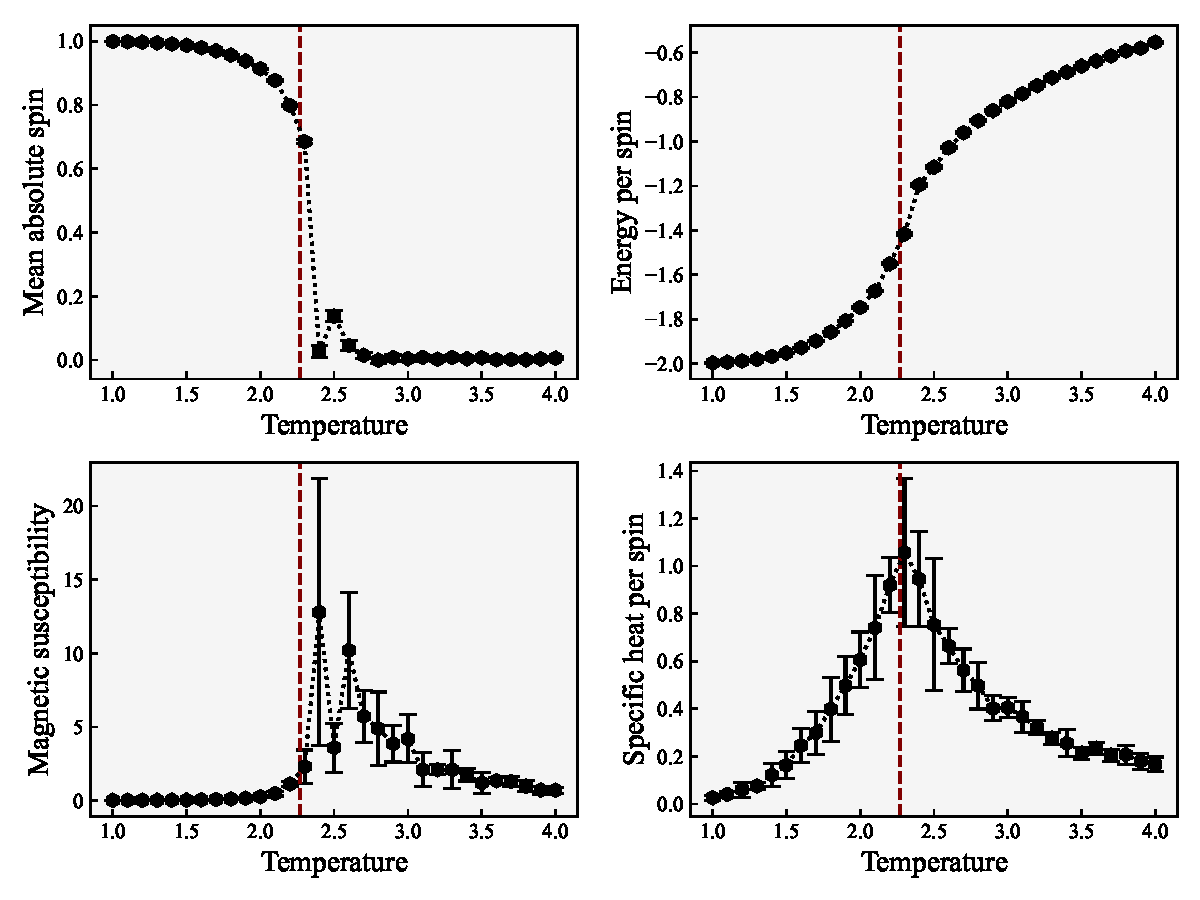
\includegraphics[width=0.75\textwidth]{figs/main_result.pdf}
    \caption{The observed mean absolute spin $\langle | m | \rangle$, energy per spin $e$, magnetic susceptibility $\chi_M$, specific heat susceptibility $C$, and their standard deviations plotted as a function of temperature. The maroon-dashed vertical line indicates the critical temperature $T_\mathrm{C}$.}
    \label{fig:fiducial}
\end{figure}

In general, our numerical experiments align very well with the theoretical models. We observe the critical temperature where it is theorised to be. After the system crosses it, the lowest-energy state shifts from the high-entropy aligned distribution to the low-entropy randomised one, increasing its energy. We draw particular attention to the sharp peak the specific heat capacity curve exhibits, as it reproduces Osnager's original, analytic solution well. It is shown in Fig.\ref{fig:osnager}.

\begin{figure}[H]
    \centering
    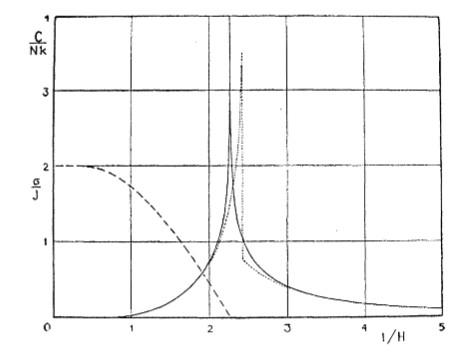
\includegraphics[width=0.45\textwidth]{figs/osnager.png}
    \caption{The solid line depicts Onager's original analytic solution for the heat capacity, Osnager (1944) \cite{Onsager}. }
    \label{fig:osnager}
\end{figure}

The uncertainties increase considerably when we approach the critical temperature. This can be traced back to the auto-correlation time, which rises almost by an order of magnitude for lattices close to $T_\mathrm{C}$.

\begin{figure}[H]
    \centering
    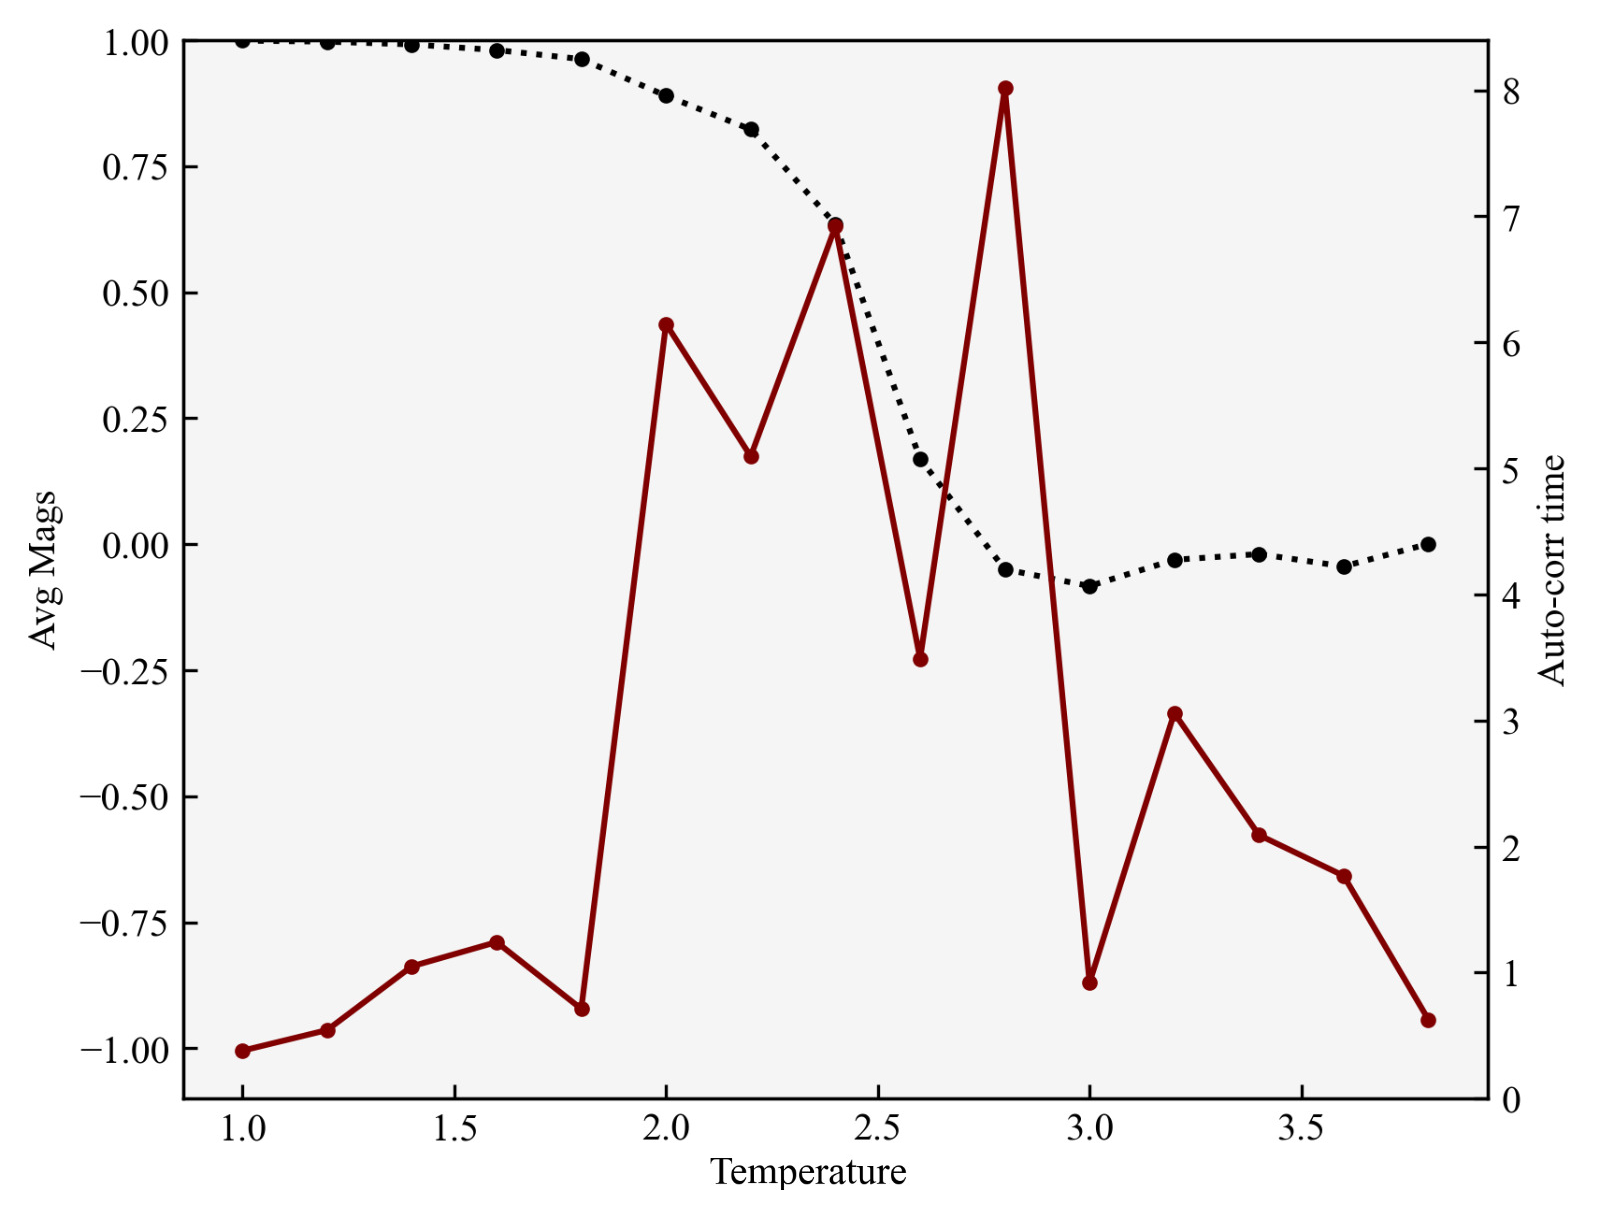
\includegraphics[width=0.55\textwidth]{figs/autocorr.png}
    \caption{The black line is the average magnetisation and the maroon line is the auto-correlation line.}
    \label{fig:enter-label}
\end{figure}

The only deviation from the theoretically expected results, is that the peak of the magnetic susceptibility does not coincide with the critical temperature, but rather occurs slightly after. The large errors for these calculations do account for that mismatch, but it is not unprecedented. Experimentally determined magnetic susceptibility curves also exhibit this behaviour, as is evident in Fig. \ref{fig:sus}.


\begin{figure}[H]
    \centering
    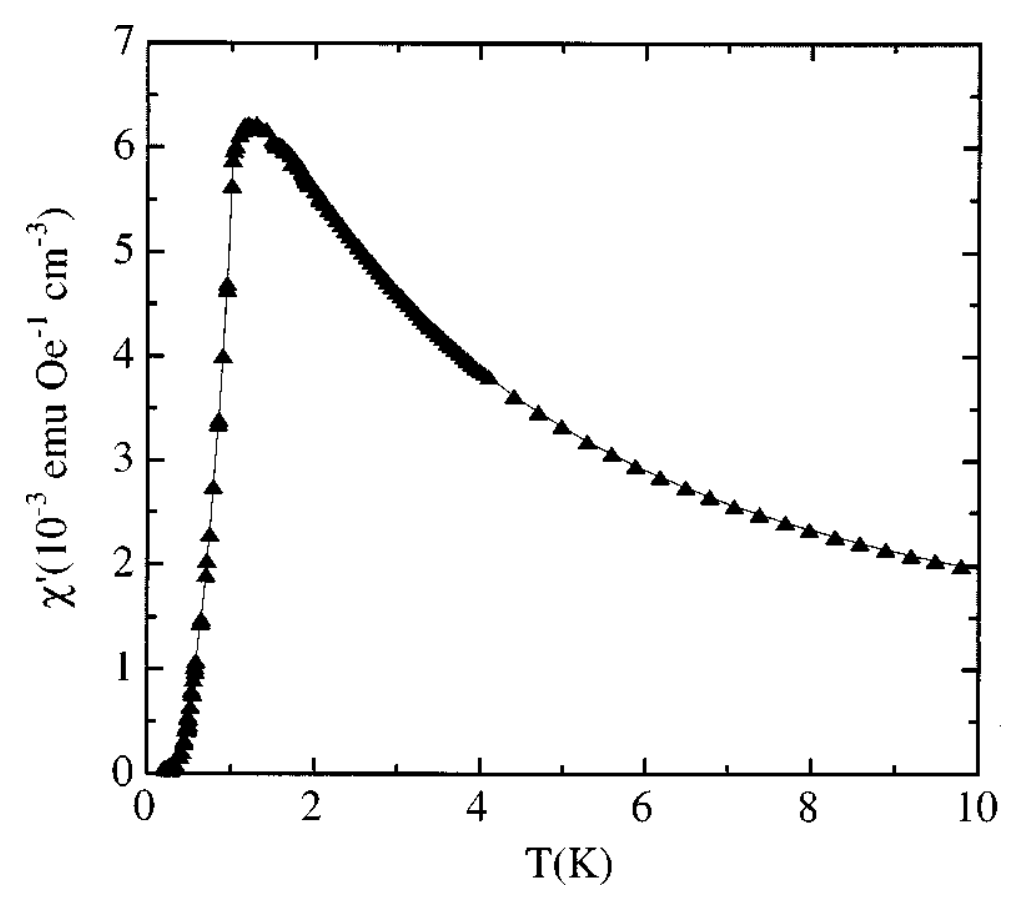
\includegraphics[width=0.55\textwidth]{figs/Mag-SUS.png}
    \caption{Experimentally determined magnetic susceptibility of NdGaO$_{3}$ \cite{magsus}. The critical temperature occurs at approximately 0.97 K.}
    \label{fig:sus}
\end{figure}

\raggedbottom
\newpage

\subsection{Non-Zero External Field}
In the presence of an external magnetic field, we still expect the existence of a phase transition. However, the critical temperature at which it occurs is much greater. We present the same observed quantities for 5 external fields but we allow the lattice to reach much hotter temperatures. In this set of simulations, we initialised the grid with 75\% positive spins. We found no significant difference when comparing to the 75\% negative spin case. A comparative figure can be found in Appendix \ref{sec: All In One}.

\begin{figure}[H]
    \centering
    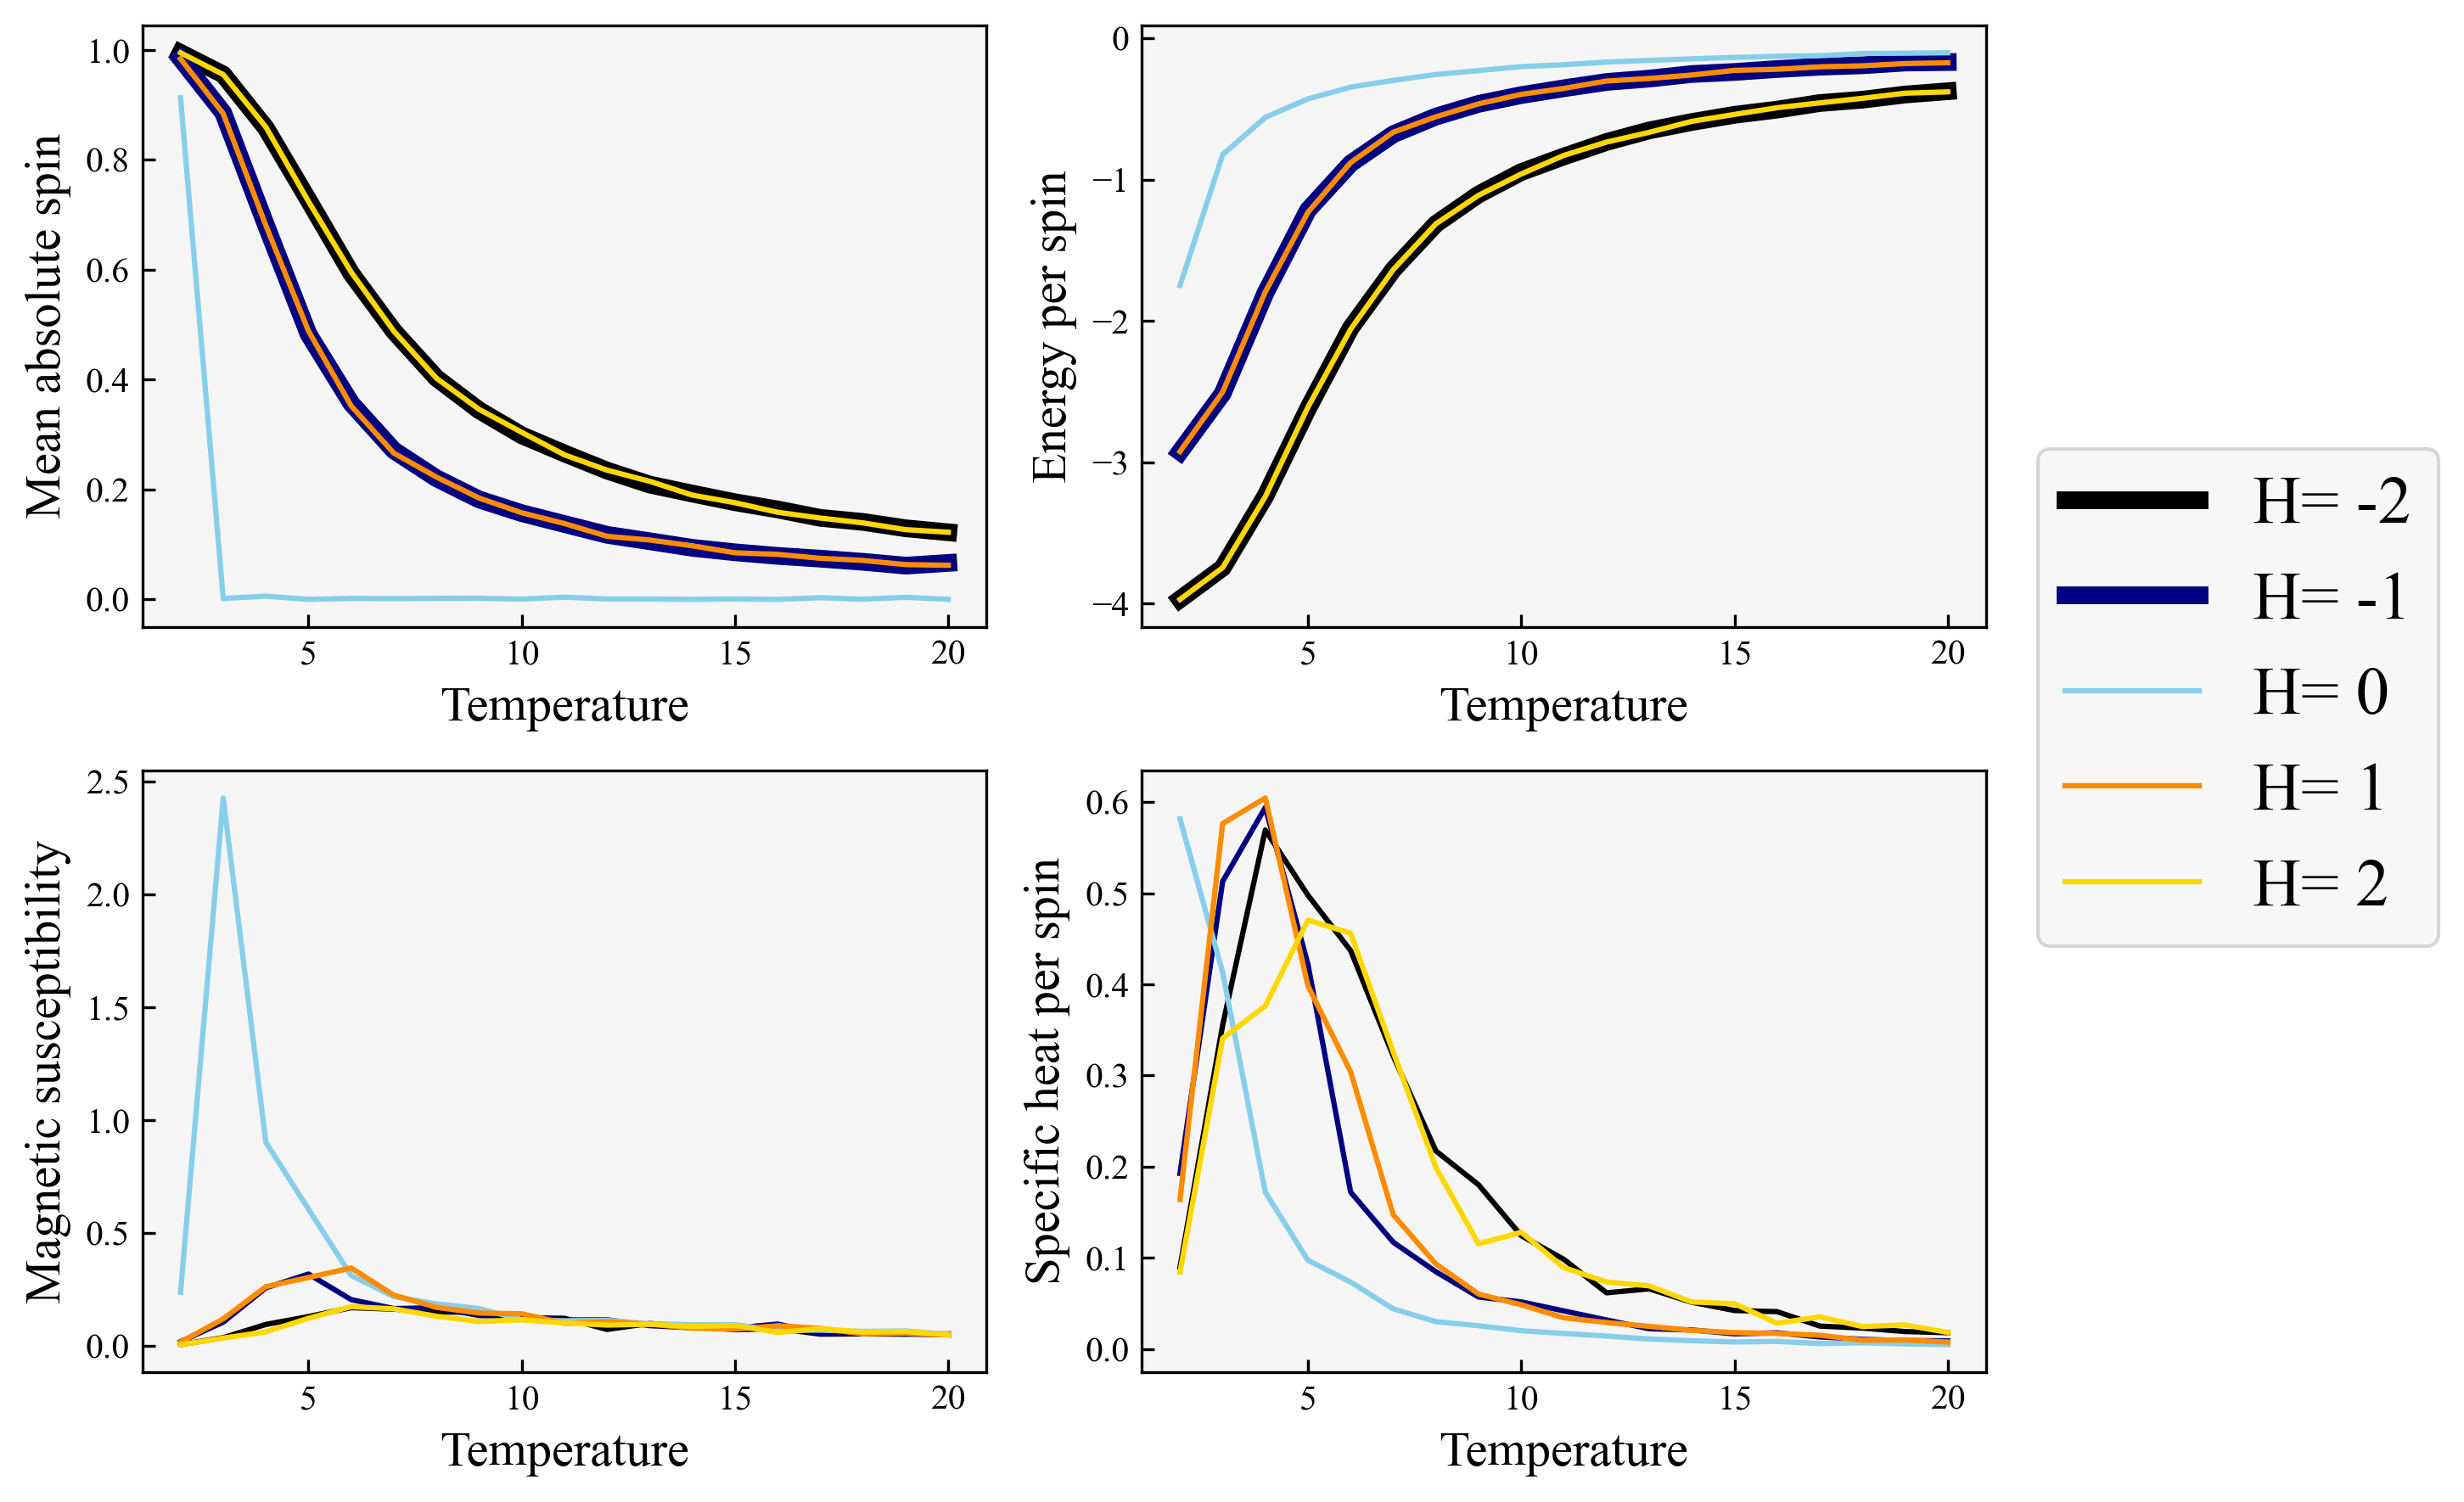
\includegraphics[width=1\textwidth]{figs/hall.png}
    \caption{The mean absolute spin, mean energy, magnetic susceptibility and specific heat for non-zero external magnetic fields. Uncertainties are not show}
    \label{fig:nonzero}
\end{figure}

It is clear that the nature of the phase transition changes. It not only requires very hot systems but it stops being discontinuous. The ferromagnet gradually loses its magnetic properties as the spins are less able to keep one another in line. The transition region increases with the strength of the magnetic field, as does $T_\mathrm{C}$. Whether or not the system begins aligned with the external field is of no consequence, as long as the temperature is high enough to allow for non-degenerate simulations. For systems with temperatures less than 2, we observed lattices immediately aligning themselves with the external field, only rarely going to higher energy states.

\raggedbottom
\newpage

\section{Summary}
\label{sct: Summary}

In this project we successfully simulated a two-dimensional ferromagnet through a  Monte-Carlo model. To that end, we implemented the Metropolis-Hastings algorithm. We observed a phase transition in the neighbourhood of temperature that theory predicts. At the critical temperature we also observed major increases in magnetic susceptibility and heat capacity.\\
We extended our investigation to systems embedded in an external magnetic field. We observed a strong rise in $T_\mathrm{C}$, scaling with the strength of the external field. The systems still exhibits a phase-transitions, but they occur at much higher temperatures, and is far more continuous. 

\bibliographystyle{siam}
%\nocite{*} % show all citations, regardless if they're used in the report.

\section*{Bibliography}
{
\renewcommand{\clearpage}{} 
\begingroup
\renewcommand{\section}[2]{}%
\bibliography{References}
\endgroup
}

\raggedbottom
\newpage

\appendix

\section{Appendix: Deriving the equation for Energy difference}
\label{sec: Proof}

Eqn. \ref{eqn: Energy Difference} gives the energy difference between two consecutive states of the lattice during the execution of the Metropolis-Hastings algorithm,

\begin{equation}
    \mathcal{H}^{\prime}-\mathcal{H}=2\left[ J \left(s_l+s_r+s_t+s_b\right)+ H\right]s_k.
\end{equation}

This relation can be derived by starting from the Hamiltonian given in Eqn. \ref{eqn: Hamiltonian},

\begin{equation}
    \mathcal{H} = -J\sum_{\langle i,j\rangle} s_is_j - H \sum_i s_i,
\end{equation}

which consists of two parts, the coupling term $C=J\sum_{\langle i,j\rangle} s_is_j$ and the total magnetisation term $M=H \sum_i s_i$. We will consider what happens to each of these parts when some spin $s_k$ is flipped,

\begin{equation}
    s_k' = -s_k,
\end{equation}

with the direct neighbours of this spin given by $s_l$,\;$s_r$,\;$s_t$,\; $s_b$. We start with the total magnetisation term $M$. Written out it is given by,

\begin{equation}
    M = H\left(s_1 + \cdots + s_k + s_l + s_r + s_t + s_b + \cdots + s_{N^2} \right).
\end{equation}

All but the $s_k$ spin remain the same, giving, 

\begin{equation}
    M' = H\left(s_1 + \cdots - s_k + s_l + s_r + s_t + s_b + \cdots + s_{N^2} \right).
\end{equation}

If we add $2Hs_k$ to $M'$, we get the expression for $M$ again. Hence,

\begin{equation}
    M' = M - 2Hs_k.
\end{equation}

The coupling term $C$ is more complicated. We will write it in the following way,

\begin{equation}
    C = J\sum_{\langle i,j\rangle} s_i s_j = \frac{J}{2}\sum_i s_i \sum_{j} s_{i,j} = \frac{J}{2}\sum_i C_i,
\end{equation}

where the factor $\frac{1}{2}$ appears to prevent double counting the same spin-pairs, and the sum $\sum_j s_{i,j}$ indicates the spin-sum of the direct neighbours of spin $s_i$. The term $C_i$ is thus given by $C_i = s_i (s_{i,l} + s_{i,r} + s_{i,t} + s_{i,b})$, $C_i$ is the individual coupling strength for each spin $s_i$ and its immediate neighbours. We start our analysis of how $C$ changes, because of a spin-flip, by analysing the change in $C_i$. 

\raggedbottom
\newpage

The vast majority of the $C_i$ values we do not have to consider, since they do not contain the flipped spin $s_k$, and hence remain constant. There are only 5 values of $C_i$ we do have to consider:

\begin{itemize}
\item  The value of $C_k$, where we calculate the coupling strength of the flipped spin $s_k$,

\begin{equation}
    C_k = s_k (s_{l} + s_{r} + s_{t} + s_{b})
\end{equation}

It is easy to see that when $s_k$ flips we simply get that,

\begin{equation}
    C_k' = -C_k.
\end{equation}

\item The values of the four $C_j$, for the immediate neighbours of $s_k$, since these are the only $C_i$ which include $s_k$,

\begin{equation}
    C_j = s_j(s_{k} + s_{j,r} + s_{j,t} + s_{j,b}),
\end{equation}

where, for convenience, we consider the flipped spin $s_k$ to always be 'left' with respect to the spin $s_j$, this is of course not true in reality but notation-wise it makes things easier to calculate and does not matter due to the commutativity of the summation.
When $s_k$ flips, $C_j$ becomes,

\begin{equation}
    C_j' = s_j(-s_{k} + s_{j,r} + s_{j,t} + s_{j,b}),
\end{equation}

similar in our calculations for $M'$, we can see that this equals,

\begin{equation}
    C_j' = C_j - 2s_js_k.
\end{equation}

\end{itemize}

Now we can tackle the total coupling term $C$. Fully written out, it is given by,

\begin{equation}
    C = \frac{J}{2}\left(C_1 + \cdots + C_k + C_l + C_r + C_t + C_b + \cdots + C_{N^2} \right).
\end{equation}

When the spin $s_k$ flips this changes to,

\begin{equation}
    C' = \frac{J}{2}\left(C_1 + \cdots + C_k' + C_l' + C_r' + C_t' + C_b' + \cdots + C_{N^2} \right).
\end{equation}

We can replace the $C_i'$ values with the expressions we derived, this simplifies to,

\begin{equation}
    C' = \frac{J}{2}\left(C_1 + \cdots -C_k + C_l + C_r + C_t + C_b -2s_k(s_l + s_r + s_t + s_b)  + \cdots + C_{N^2} \right).
\end{equation}

\raggedbottom
\newpage

The term $-2s_k(s_l + s_r + s_t + s_b)$ simply equals $-2C_k$, as per our definition of $C_i$,

\begin{equation}
    C' = \frac{J}{2}\left(C_1 + \cdots -3C_k + C_l + C_r + C_t + C_b  + \cdots + C_{N^2} \right).
\end{equation}

We add and subtract a $C_k$ term inside the parentheses to get our expression for $C$ back, this results in a $-4C_k$ term inside the parentheses, which gives our final expression for total coupling term after spin-flip $C'$,

\begin{equation}
    C' = C - 2JC_k.
\end{equation}

We can now derive our expression for the energy difference between consecutive states. We write the Hamiltonian as,

\begin{equation}
    \mathcal{H} = -C -M.
\end{equation}

The Hamiltonian after spin-flip is thus,

\begin{equation}
    \mathcal{H}' = -C' - M',
\end{equation}

subtracting the expression for the Hamiltonian before spin flips gives the energy difference between consecutive states,

\begin{equation}
    \mathcal{H}' - \mathcal{H} = -(C'- C) - (M'-M).
\end{equation}

Substituting in our derived expressions for $C'$ and $M'$ we get,

\begin{equation}
    \mathcal{H}' - \mathcal{H} = 2JC_k +2Hs_k.
\end{equation}

Finally, we substitute in our expression for $C_k = s_k (s_{l} + s_{r} + s_{t} + s_{b})$ to get Eqn. \ref{eqn: Energy Difference},

\begin{equation}
    \mathcal{H}^{\prime}-\mathcal{H}=2\left[ J \left(s_l+s_r+s_t+s_b\right)+ H\right]s_k.
\end{equation}

\raggedbottom
\newpage

\section{Appendix: Non-Zero External Field}
\label{sec: All In One}

\begin{figure}[H]
    \centering
    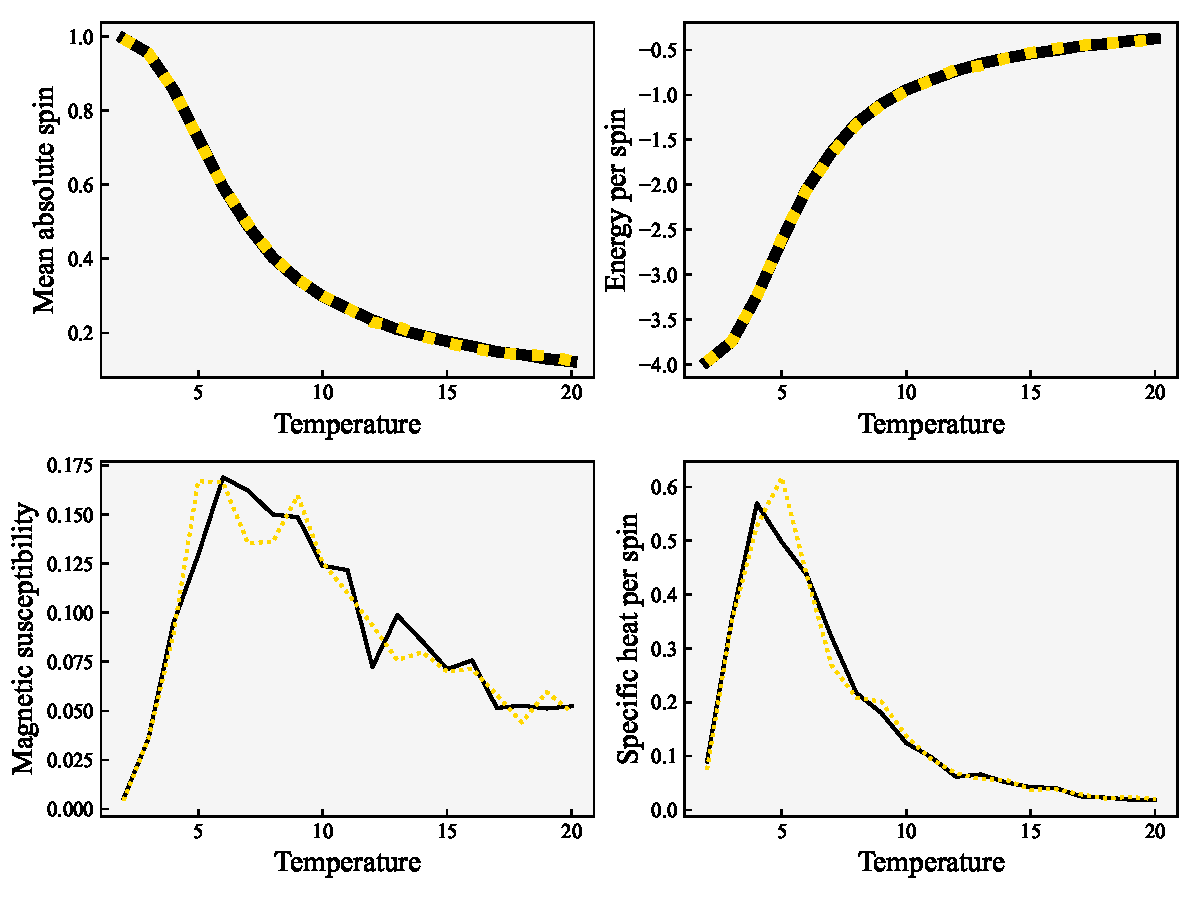
\includegraphics[width=1\textwidth]{figs/nonzeroHall.pdf}
    \caption{The observable quantities for $H=-2$. The different colours correspond to different grids initialisation. Either 75\% positive spin (black) or 75\% negative spin (gold).}
    \label{fig:enter-label}
\end{figure}

\end{document}
